% !TEX root = main.tex
%%%%%%%%%%%%%%%%%%%%%%%%%%%%%%%%%%%%%%%%%%%%%%%%%%%%%%%%%%%%%%%%%%%%%%%%%%%%%%%%
% Data Collection and Preprocessing
%%%%%%%%%%%%%%%%%%%%%%%%%%%%%%%%%%%%%%%%%%%%%%%%%%%%%%%%%%%%%%%%%%%%%%%%%%%%%%%%
\section{Data Collection and Preprocessing}
\label{section:dataprep}
Data on Titan GPU life times is constructed from two sources:
inventory runs and failure event \rev{log} records. Two types of
failure events were collected \rev{for this study}: Double Bit Error
(DBE) and Off the Bus (OTB). \rev{DBE is a memory error detected by
  parity bit checking, which can correct a single bit flip and detect
  but not correct a double bit flip. OTB is the loss of host CPU
  connection to the GPU. While other types of errors were recorded in
  log files, as is reported in \cite{7266836,tiwari15Understand}, OTB
  and DBE became dominant in 2016 and were found to be the
  ``signature'' event of the GPU board failing resistor and a trigger
  for GPU replacement.}

An inventory of GPU serial numbers and their locations was recorded
each time the system boots, \rev{typically for software updates and
  patches but sometimes for hardware swaps, although warm swaps of
  blades were usually possible.} Boots typically occured once every
few days but sometimes even a few times per day. A single inventory
takes about a minute and is recorded in a separate file. \rev{It can
  be incomplete if a node response times out but such occurrences were
  relatively rare.
\begin{figure}[bt]
  \begin{center}
    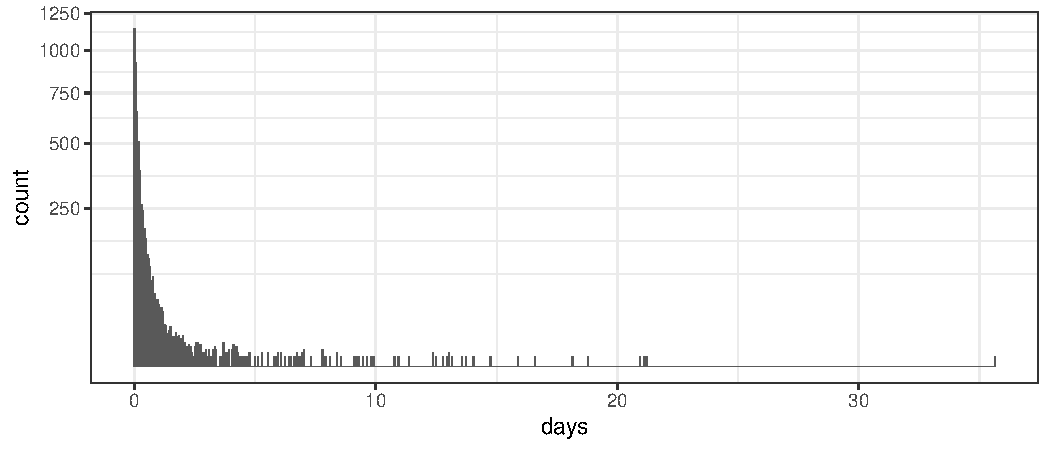
\includegraphics[width=\columnwidth]{figs/attention_intervals001.pdf}
  \end{center}
  \caption{Inter-inventory times, taken as time intervals between
    unique dates in the data and removing those less than a day.}
  \label{fig:inventory}
\end{figure}
Figure~\ref{fig:inventory} shows that during 2014 and 2015,
inventories were far apart, even 56 days once in 2014. The purpose is
to illustrate that exact times for GPU removal from service are
``censored'' and we only get the inventory time information. We discuss
censoring and its implications in Sec.~\ref{section:survival}.}

Initial processing updates an inventory by checking the Serial Number
(\rev{{\em SN}}) and Location of each GPU and creating or updating a
separate record for each contiguously observed
\rev{{\em{SN-Location}}} combination. Resulting GPU data records are
of the form shown in Fig.~\ref{fig:dataraw},
\begin{figure}[tb]
{\notsotiny
\begin{verbatim}
0323812007945 | c17-4c1s3n1 | 01/10/2013 02:54:45 | 02/02/2013 11:32:29
 | c13-1c1s3n3 | 01/21/2014 21:10:42 | 08/01/2017 02:15:02
 | c0-1c1s3n3 | 10/11/2013 15:57:33 | 10/12/2013 22:09:31
 | c21-1c2s5n0 | 03/19/2013 15:48:11 | 05/29/2013 11:54:11
0325216047736 | c18-4c1s5n1 | 03/07/2017 02:15:01 | 03/12/2019 03:19:11
0323812008856 | c5-4c0s7n0 | 01/10/2013 02:54:45 | 01/25/2013 15:29:58
 | c0-6c1s7n2 | 10/21/2013 14:28:19 | 10/28/2013 17:52:44
 | c3-3c1s5n0 | 05/29/2013 11:54:11 | 05/29/2013 11:54:11
 | c23-6c1s7n2 | 01/21/2014 21:10:42 | 11/02/2018 14:42:34
 | | DBE | 11/02/2018 14:42:34
\end{verbatim}
}
\caption{A few records of raw data produced from inventories \rev{and
    log files} that is processed further in our analysis.}
\label{fig:dataraw}
\end{figure}
where records for three are shown. Each record starts with a serial
number and locations are coded with {\tt c{\it col-row}c{\it
    cage}s{\it slot}n{\it node}}. The location references are cabinet
column (0-24), row (0-7), cage (0-2), slot (0-7), and node (0-3) with
respect to the layout shown in \rev{Fig.}~\ref{fig:layout}. \rev{Note
  that there is an extra empty column of cabinets between columns 10
  and 11 to accommodate a few ceiling support columns. To aid
  orientation in the figure, we mark an example location {\tt
    c17-4c1s3n1} with a yellow dot in each view of the figure.}
\begin{figure}
  \centering
  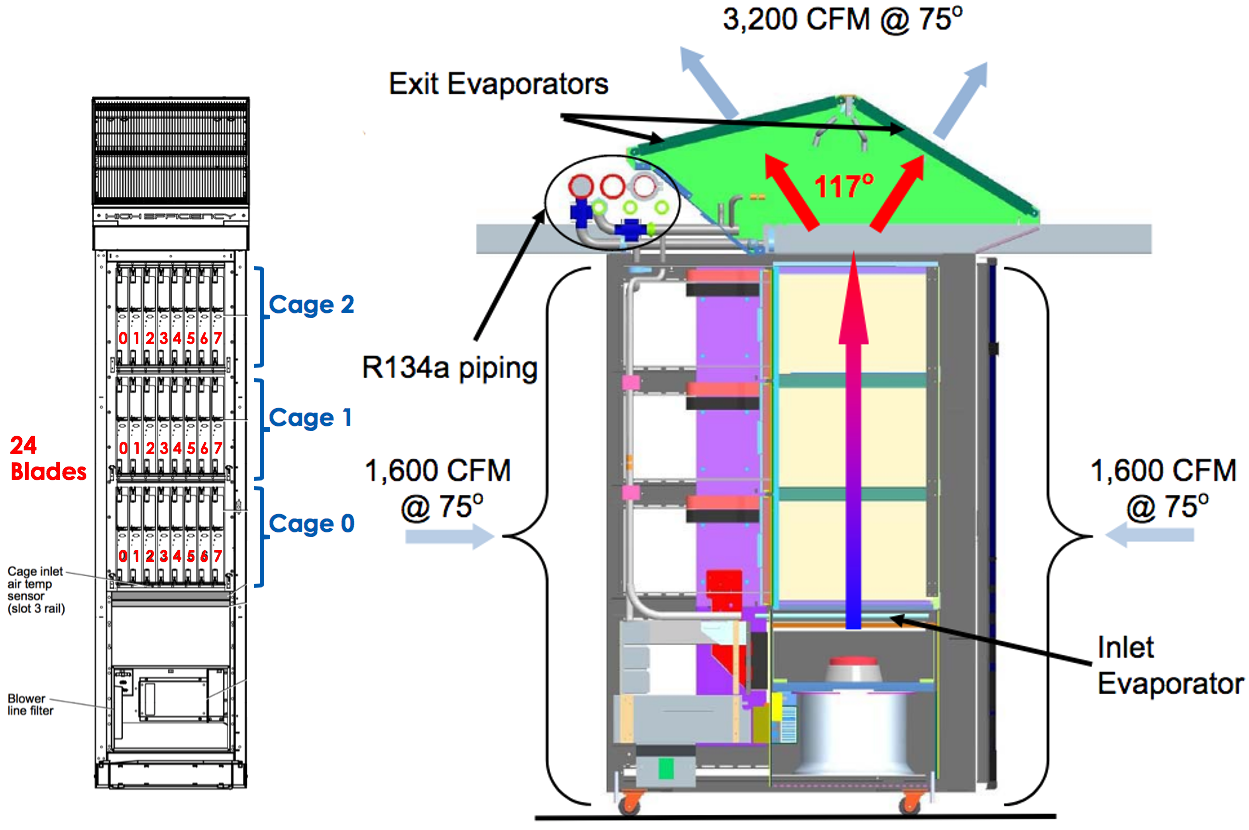
\includegraphics[width=\columnwidth]{figs/TitanCabinet.png}
  \begin{minipage}{0.35\columnwidth}
    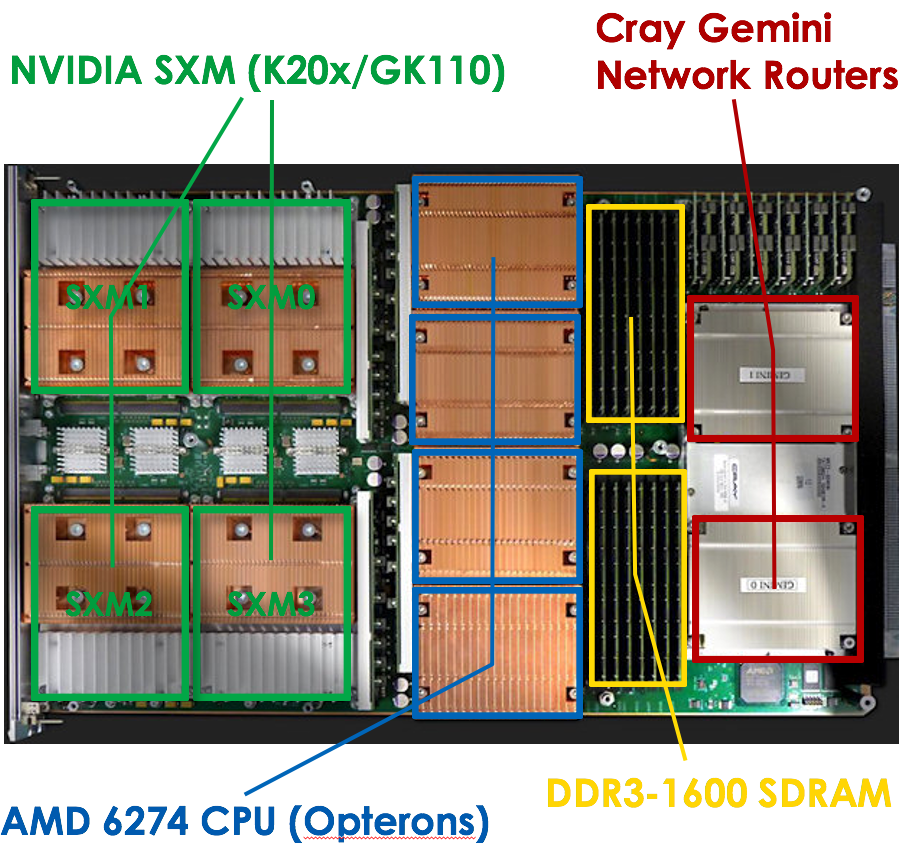
\includegraphics[width=\columnwidth]{figs/TitanBlade.png}
  \end{minipage}
  \hfil
  \begin{minipage}{0.49\columnwidth}
    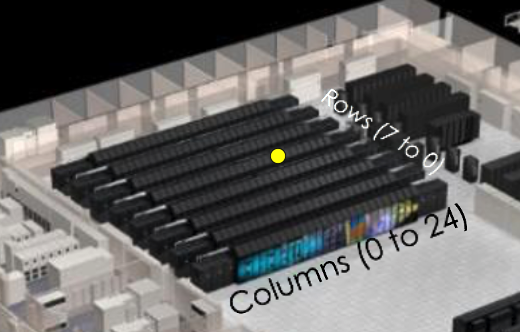
\includegraphics[width=\columnwidth]{figs/TitanLayout.png}
  \end{minipage}
  \caption{\rev{Titan cabinet (front view and side view with air flow)
      and single blade layout (bottom left with {\em node} numbers)
      and floor layout (bottom right with {\em col} and {\em row}
      numbers). Cooling airflow is bottom to top within a cabinet,
      taking ambient air in mostly at the foot and relasing it back
      out at the top. Cooling fluid is passed through heat exchange
      evaporators, below Cage 0 and above Cage 2. Ambient air in the
      room is conditioned at nominal 75$^\circ$~F. The room air system
      has a dozen intakes near the ceiling and dumps cool air under
      the floor in several locations. A number of floor tiles are
      perforated.  Yellow dot marks GPU location {\tt c17-4c1s3n1}.}}
  \label{fig:layout}
\end{figure}

The first GPU record in \rev{Fig.~\ref{fig:dataraw}} shows
installation in locations {\tt c17-4c1s3n1}, {\tt c21-1c2s5n0}, {\tt
  c0-1c1s3n3}, with periods off the system, and finally in {\tt
  c13-1c1s3n3}, where it stays until August 1, 2017, after which it is
not seen again. The second is installed in location {\tt c18-4c1s5n1},
where it stays until the last data collection date on March 3, 2019,
at 3:19:11 AM. The third GPU is first installed in locations {\tt
  c5-4c0s7n0}, {\tt c3-3c1s5n0}, {\tt c0-6c1s7n2}, and {\tt
  c23-6c1s7n2}, where a ``DBE'' is observed on November 2, 2018, and
it is not seen again. \rev{This is the data set we make publicly
  available.}

% I noticed more perforated floor tiles on the right than on the left
% in the Titan decomissioning disassembly video. Anecdotally, the
% right side of the machine was hotter than the left so some
% perforated floor tiles were moved to the right.